
\documentclass{beamer}
\usepackage{xparse}
\usepackage[latin1]{inputenc}
\usepackage{slashed}
\usepackage{amsmath}

\usepackage{amssymb}
\usepackage{amsfonts}
\usepackage{lmodern}
\mode<presentation> 
\usetheme{CambridgeUS}
\usepackage[english]{babel}
\usepackage{hyperref}
\usepackage{tabularx}
\usepackage{verbatim}
\usepackage{caption}
\captionsetup[figure]{labelformat=empty, font=tiny}% redefines the caption setup of the figures environment in the beamer class.



\begin{document}
\setbeamertemplate{bibliography item}{\insertbiblabel}
\title{Cancer Classification Challenge 2023}
\subtitle{DL4IA - Group 3}
\author{Linus Falk, Teng-Sung Yu} %add name here

\maketitle

%-----EXAMPLE SLIDES-----%

\setbeamertemplate{caption}{\raggedright\insertcaption\par}

\begin{frame}
\frametitle{Outline}
\begin{columns}
\begin{column}{0.5\textwidth}

\begin{itemize}
\setlength{\itemsep}{0.5em}
  \item What worked - Transfer learning
  \item What didn't work - Contrastive learning
  \item Results
\end{itemize}

\end{column}
\begin{column}{0.5\textwidth}  %%<--- here
\begin{center}
    \begin{figure}
    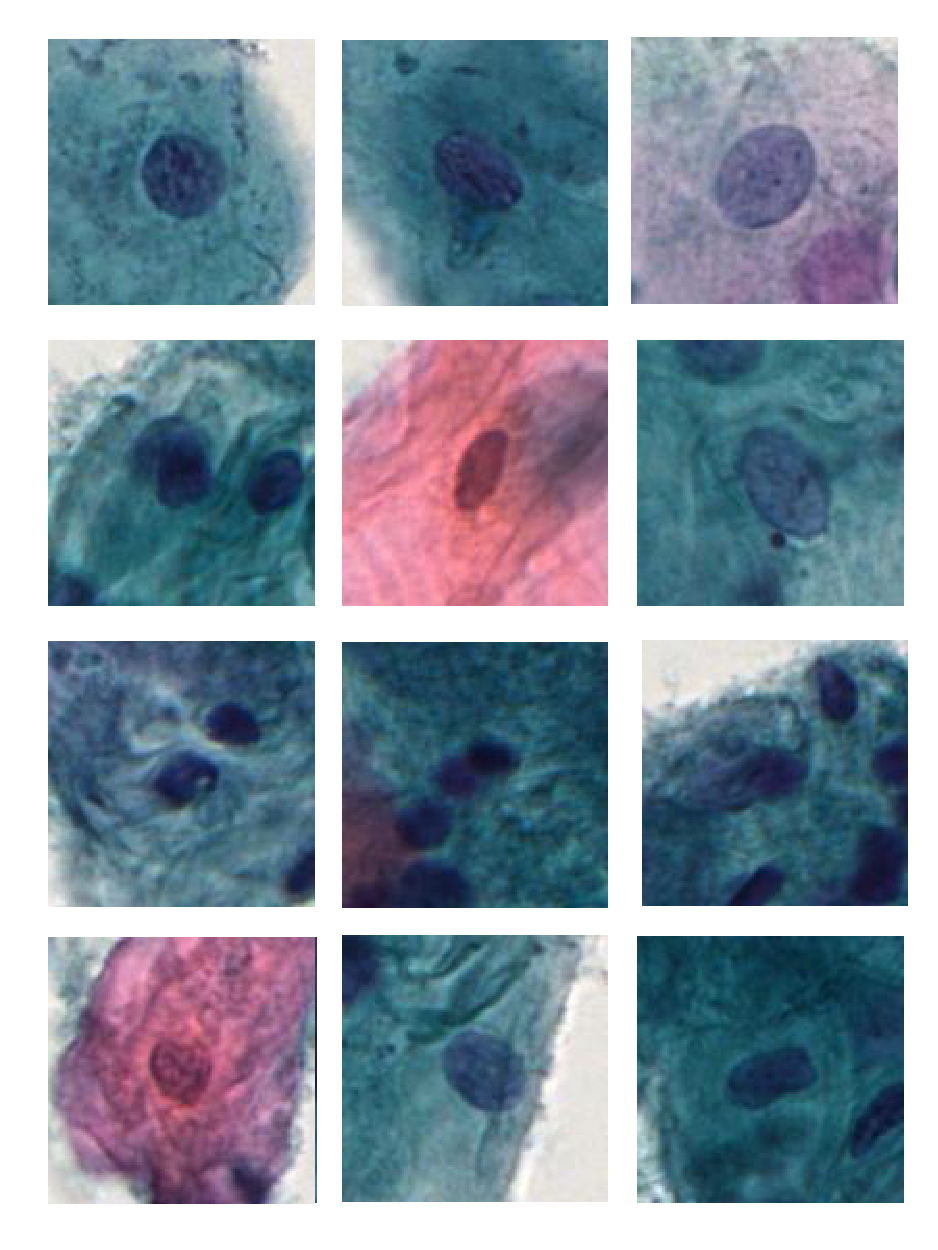
\includegraphics[width=0.7\textwidth]{figures/benignmalign.pdf}
    \caption{Benign or malignant?}
    \end{figure}
\end{center}
\end{column}
\end{columns}
\end{frame}



% ------------------------------------------------- %


\setbeamertemplate{caption}{\raggedright\insertcaption\par}

\begin{frame}
\frametitle{Transfer learning}
\begin{columns}
\begin{column}{0.5\textwidth}
\begin{itemize}
\setlength{\itemsep}{2em} 
    \item Pre-trained on ImageNet 
    \begin{itemize}
        \item ResNet50
        \item Freeze \& unfreeze layers
    \end{itemize}

    \item Learning rate strategy        \begin{itemize}
        \item Decrease step-size 90\% every 5th epoch 
    \end{itemize}
    \item Regularization

    
    \begin{itemize}
        \item Data augmentation
        \item L2
    \end{itemize}

\end{itemize}
\end{column}
\begin{column}{0.5\textwidth}  %%<--- here
\begin{center}
\begin{itemize}
    \begin{figure}
        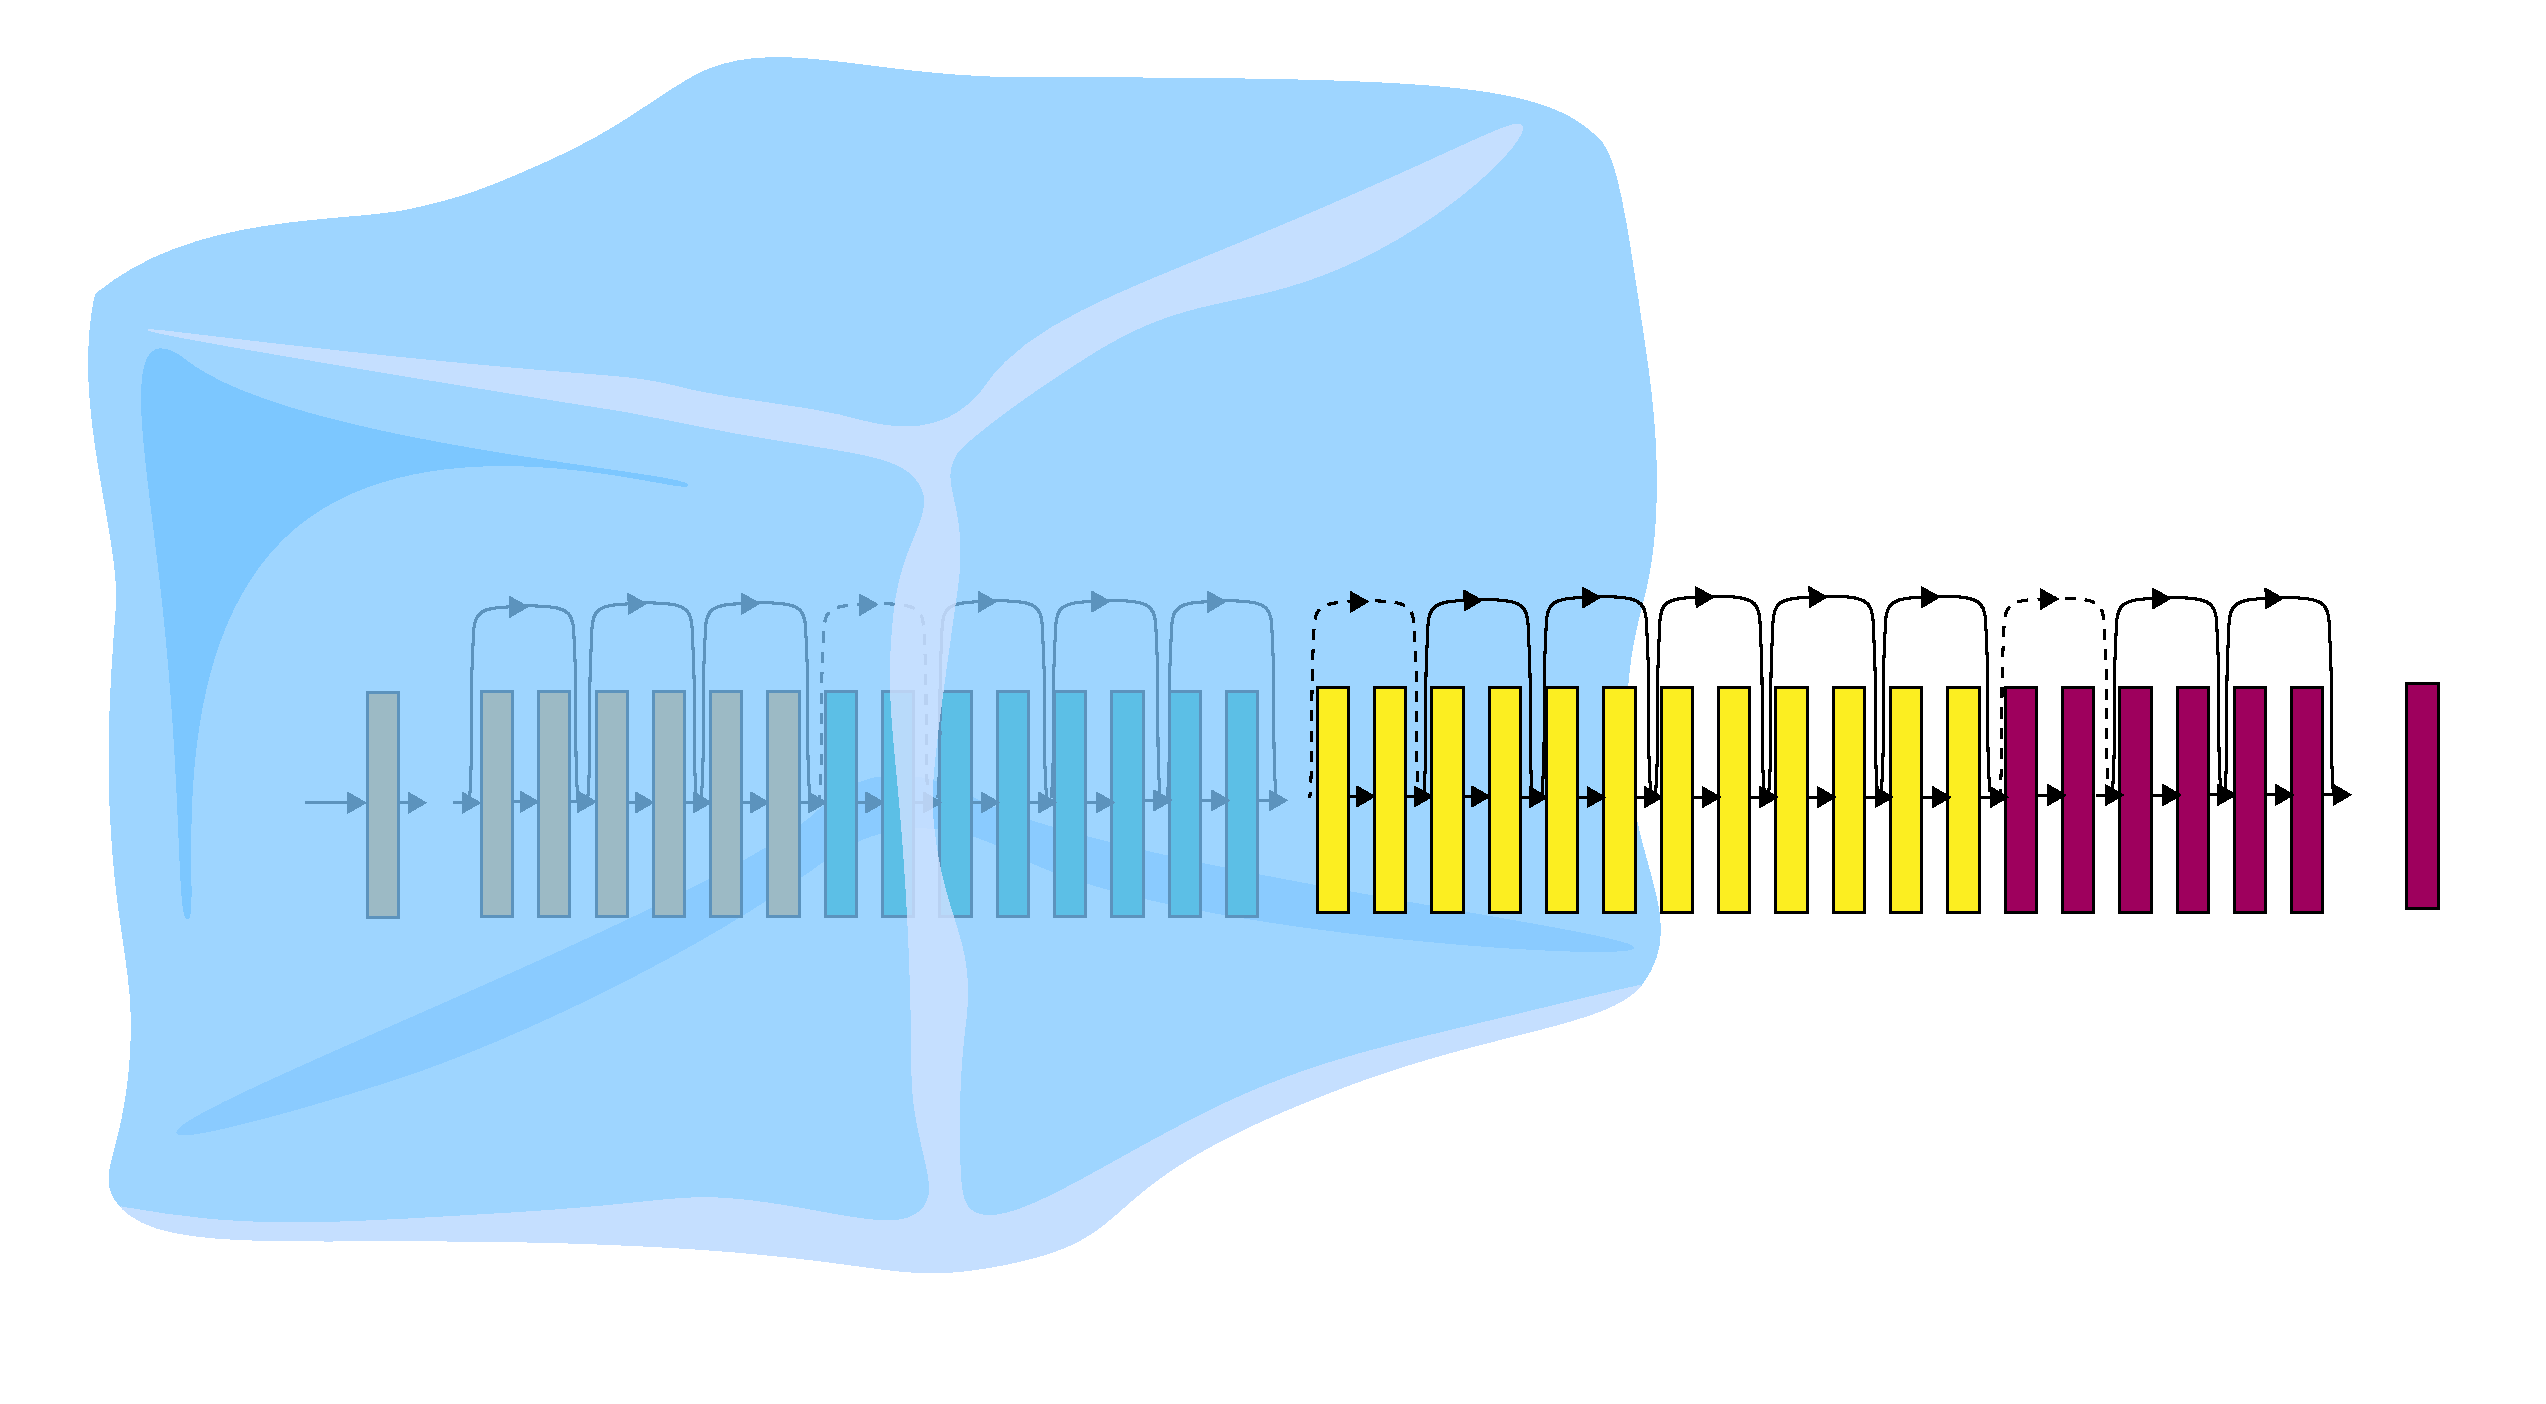
\includegraphics[width=0.7\textwidth]{figures/freeze.pdf}
    \caption{Freezing parts of ResNet}
    \end{figure}
    \begin{figure}
        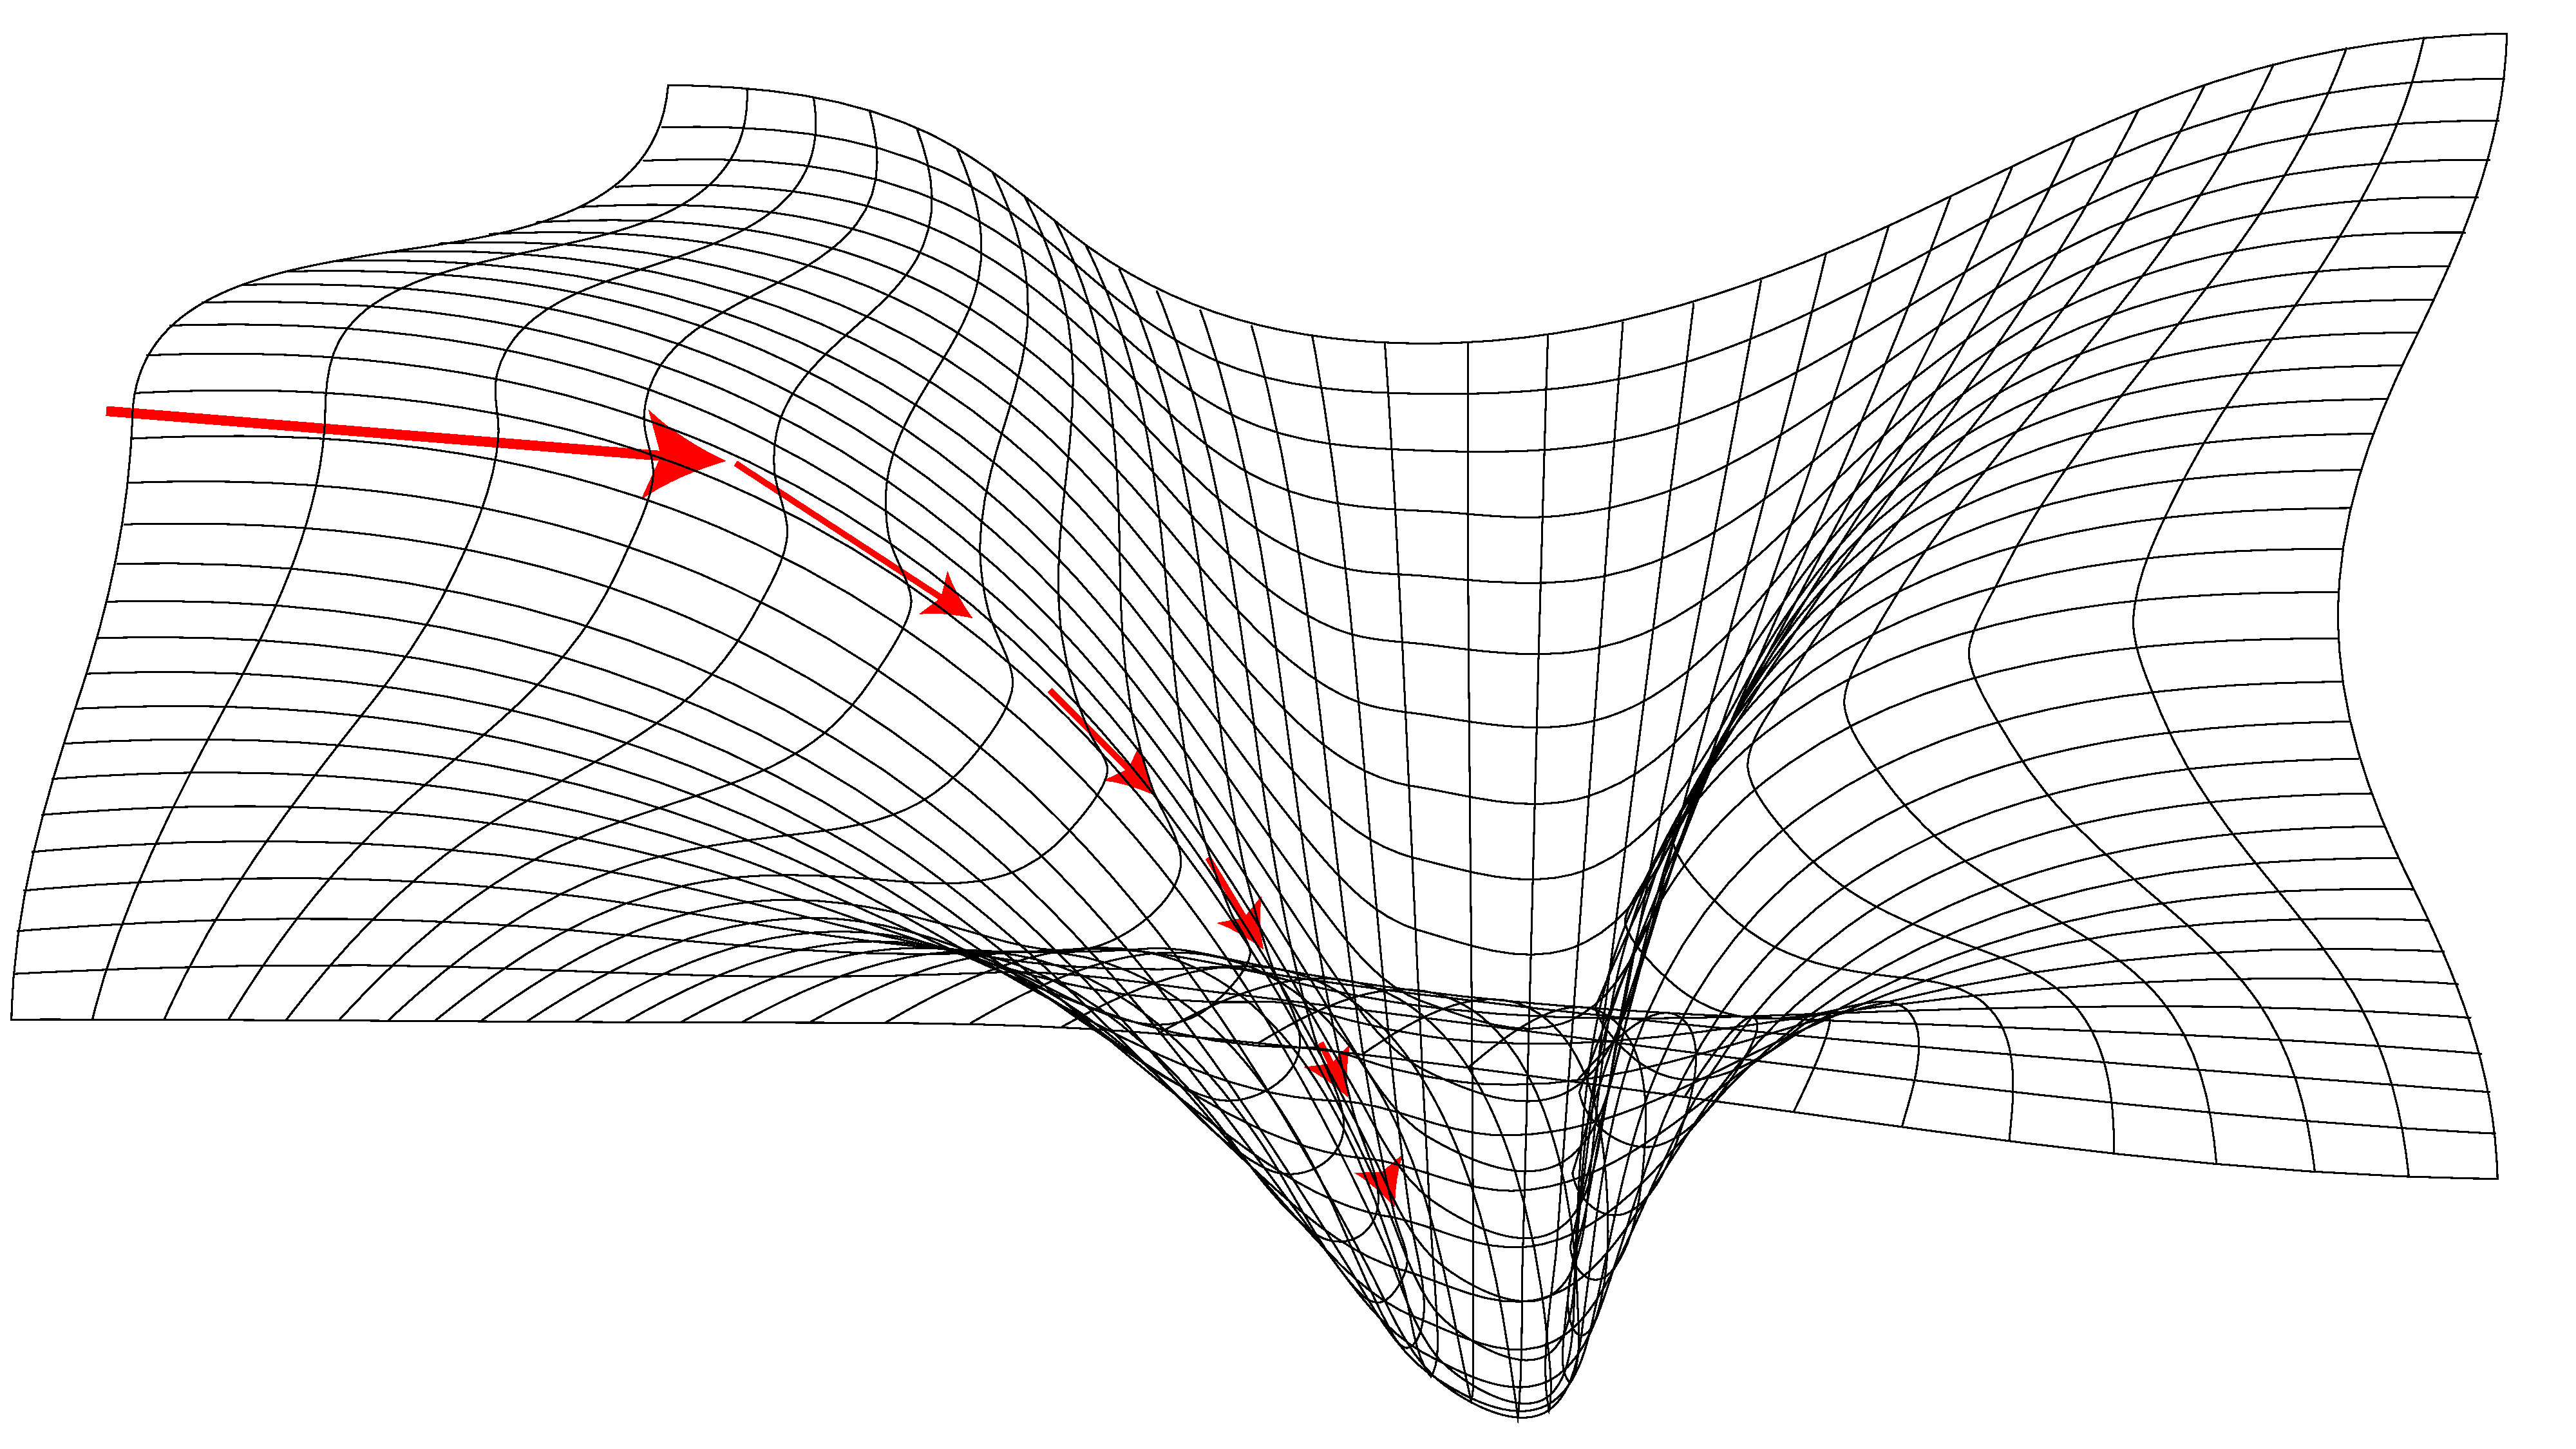
\includegraphics[width=0.9\textwidth]{figures/learningrate.pdf}
    \caption{Changing Learning Rate }
    \end{figure}   
\end{itemize}
\end{center}
\end{column}
\end{columns}
\end{frame}

% ------------------------------------------------- %


\setbeamertemplate{caption}{\raggedright\insertcaption\par}

\begin{frame}
\frametitle{Hyperparameters}
\begin{table}[]
\begin{tabular}{ll}
\hline
\textbf{Hyperparameter}        & \textbf{Value}     \\ \hline
Batch Size                     & 32                 \\
Random Rotation Range          & -45 to 45 degrees  \\
Random Resize Crop Scale Range & 0.5 to 3           \\
Loss Function                  & Cross-Entropy Loss \\
Optimizer                      & Adam               \\
Learning Rate                  & 0.1                \\
Scheduler Step Size            & 5                  \\
Scheduler Gamma                & 0.1                \\
Regularization Strength        & 0.01               \\
Number of Epochs               & 20                 \\ \hline
\end{tabular}
\end{table}
\end{frame}
% ------------------------------------------------- %

\setbeamertemplate{caption}{\raggedright\insertcaption\par}

\begin{frame}
\frametitle{Contrastive learning}
\begin{columns}
\begin{column}{0.5\textwidth}
\begin{itemize}
\setlength{\itemsep}{2em}  

    \item SimCLR 
    \begin{itemize}
        \item ResNet 50 architecture
	   \item Remove FC classification layer 
        \item Replace with Projection head \cite{SimCL}
    \end{itemize}
    \item Train on unlabeled data
    \begin{itemize}
        \item InfoNCE loss \cite{infoloss}
    \end{itemize}
    
    \item Transfer learning
    \begin{itemize}
        \item Classification head
        \item Layer-wise unfreezing
        \item Early stopping
    \end{itemize}
\end{itemize}

\end{column}
\begin{column}{0.5\textwidth}  %%<--- here
\begin{center}
\begin{itemize}
    \begin{figure}
        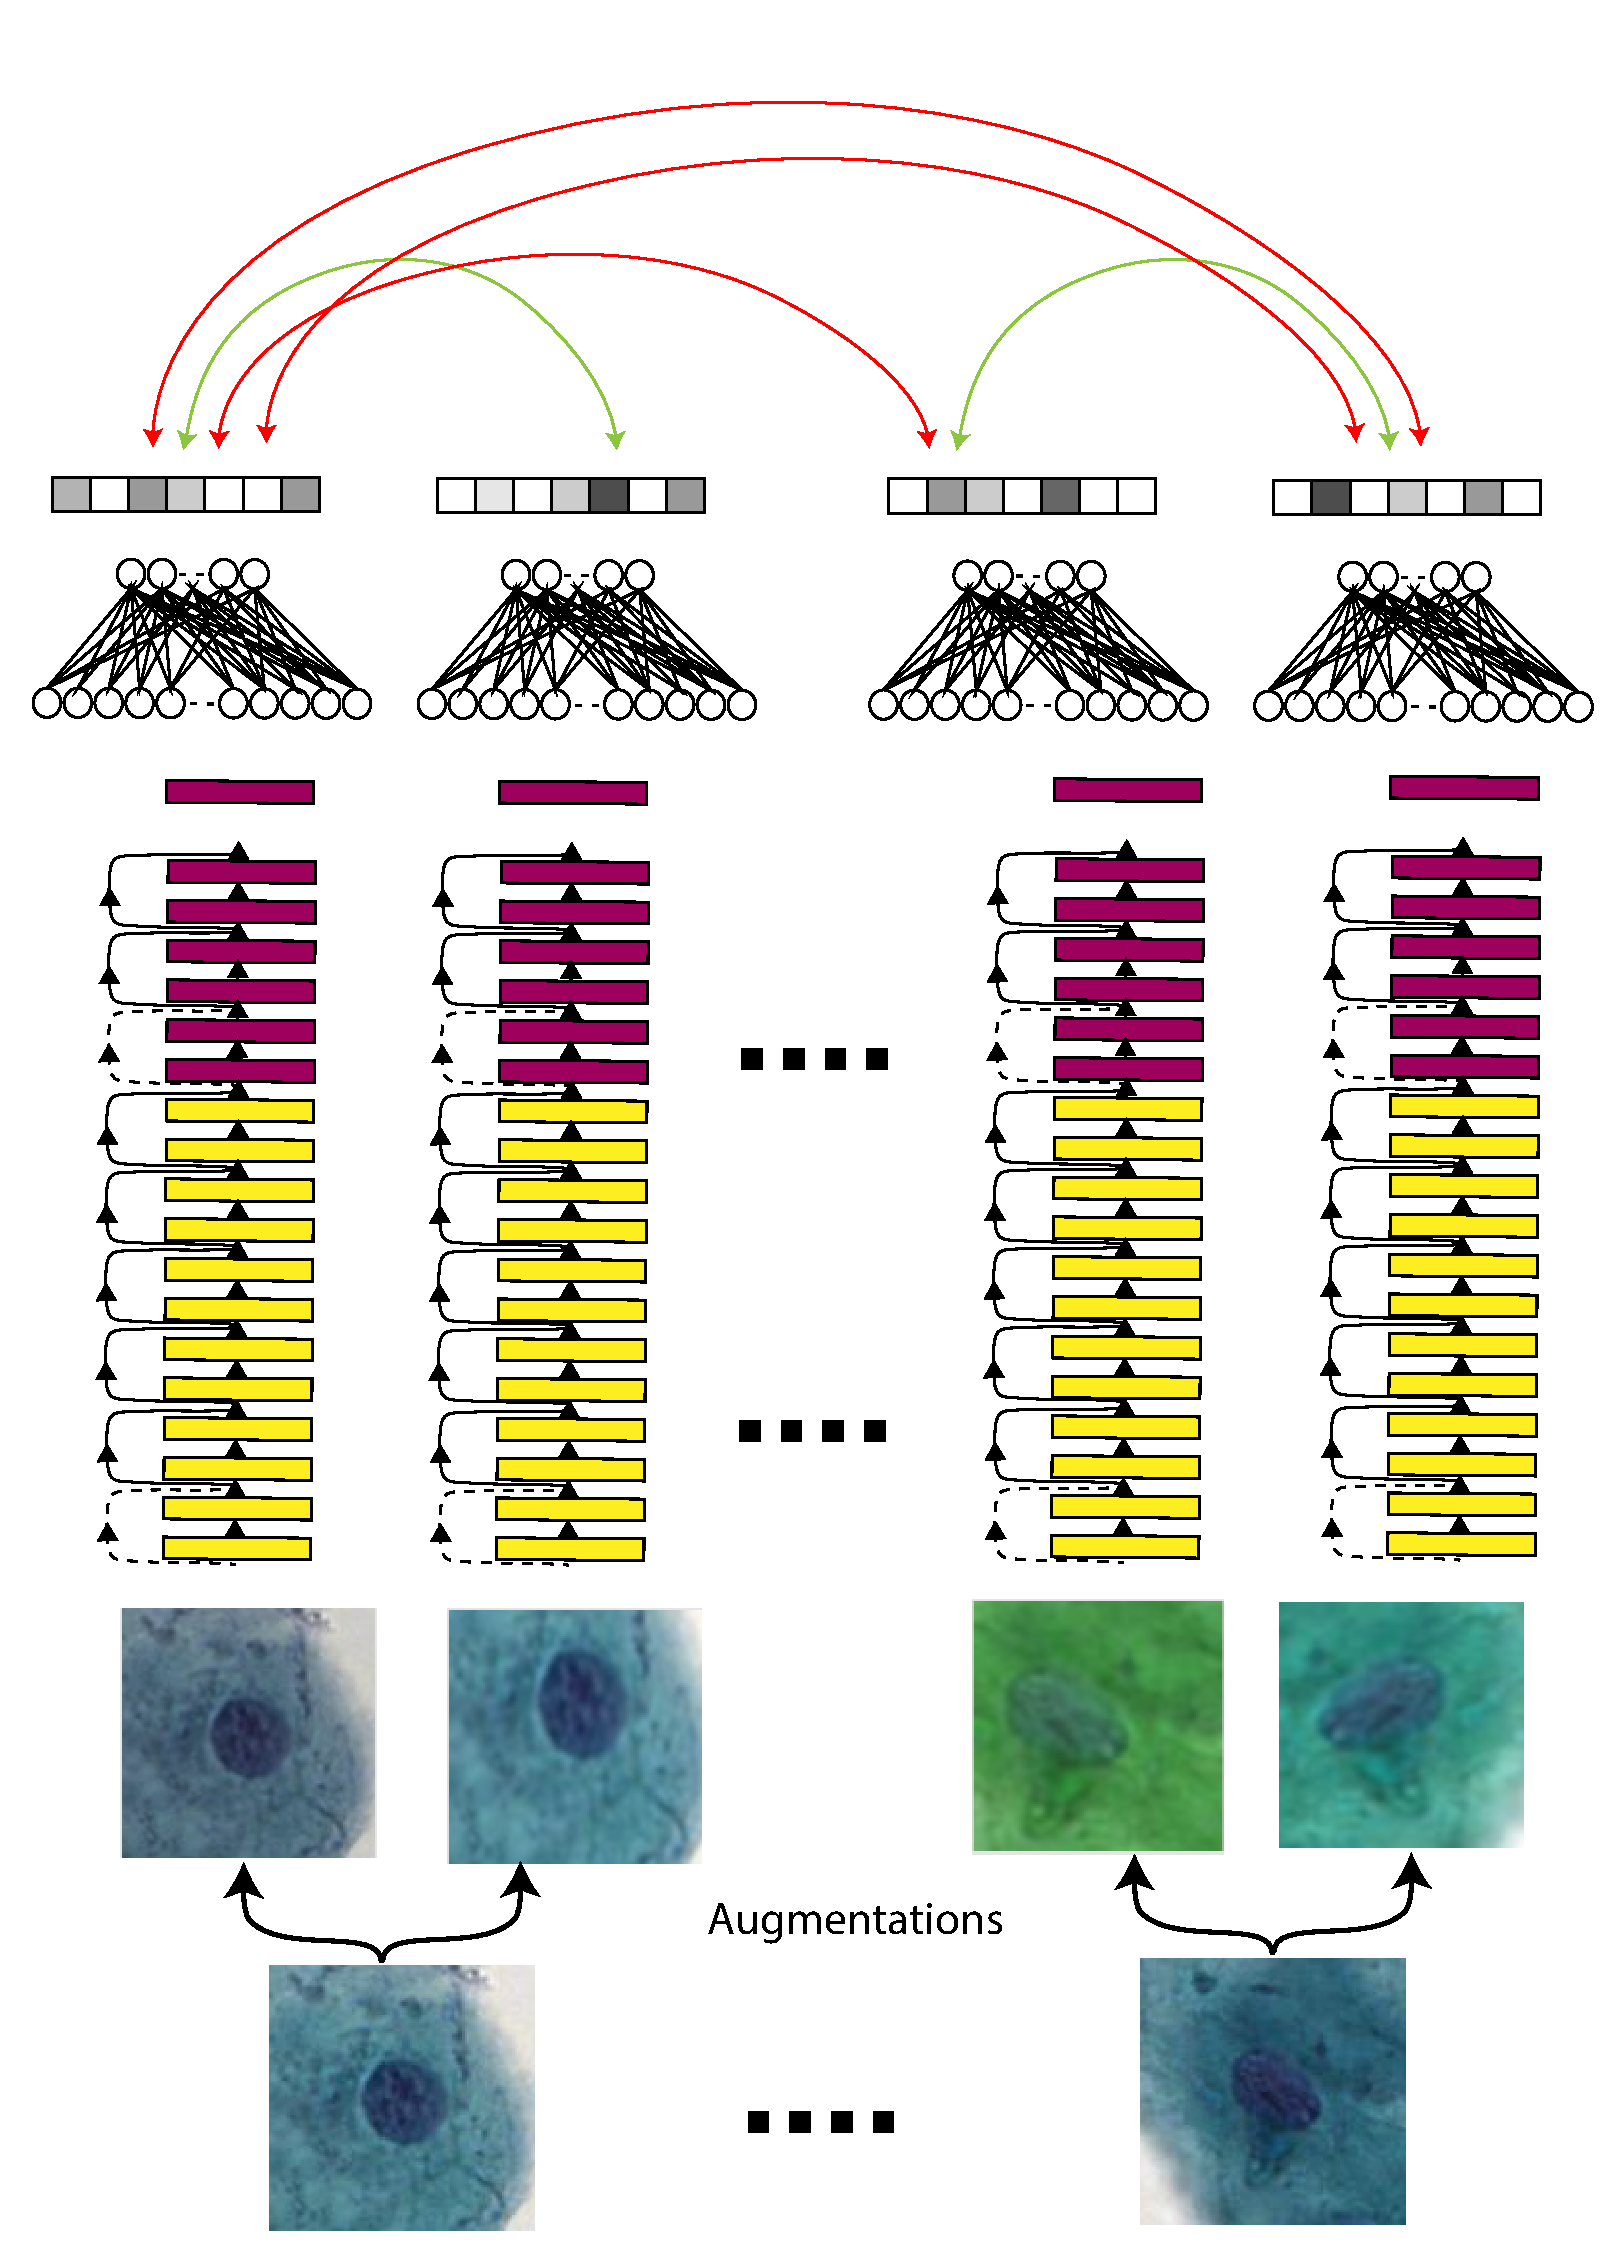
\includegraphics[width=0.8\textwidth]{figures/contastivelearning.pdf}
    \caption{}
    \end{figure}
\end{itemize}
\end{center}
\end{column}
\end{columns}
\end{frame}

% ------------------------------------------------- %

\setbeamertemplate{caption}{\raggedright\insertcaption\par}

\begin{frame}

\begin{table}[]
\begin{tabular}{ll}
\hline
\textbf{Hyperparameter} & \textbf{Value} \\ \hline
Batch Size (train, validation, test) & 16 \\
Number of Epochs & 15 \\
Initial Learning Rate & 5e-4 \\
Step Size (LR scheduler) & 3 \\
Gamma (LR scheduler) & 0.8 \\
Optimizer & Adam \\
Weight Decay (Optimizer) & 1e-3 \\
Class Weights & [0.33, 0.67] \\
Loss Function & CrossEntropyLoss \\
Transformations & HorizontalFlip, GaussianBlur, \\
& Rotation \\
& ColorJitter  \\ \hline
\end{tabular}
\end{table}

\end{frame}

% ------------------------------------------------- %

\setbeamertemplate{caption}{\raggedright\insertcaption\par}

\begin{frame}
\frametitle{A lot of training later ....}

    \begin{figure}
        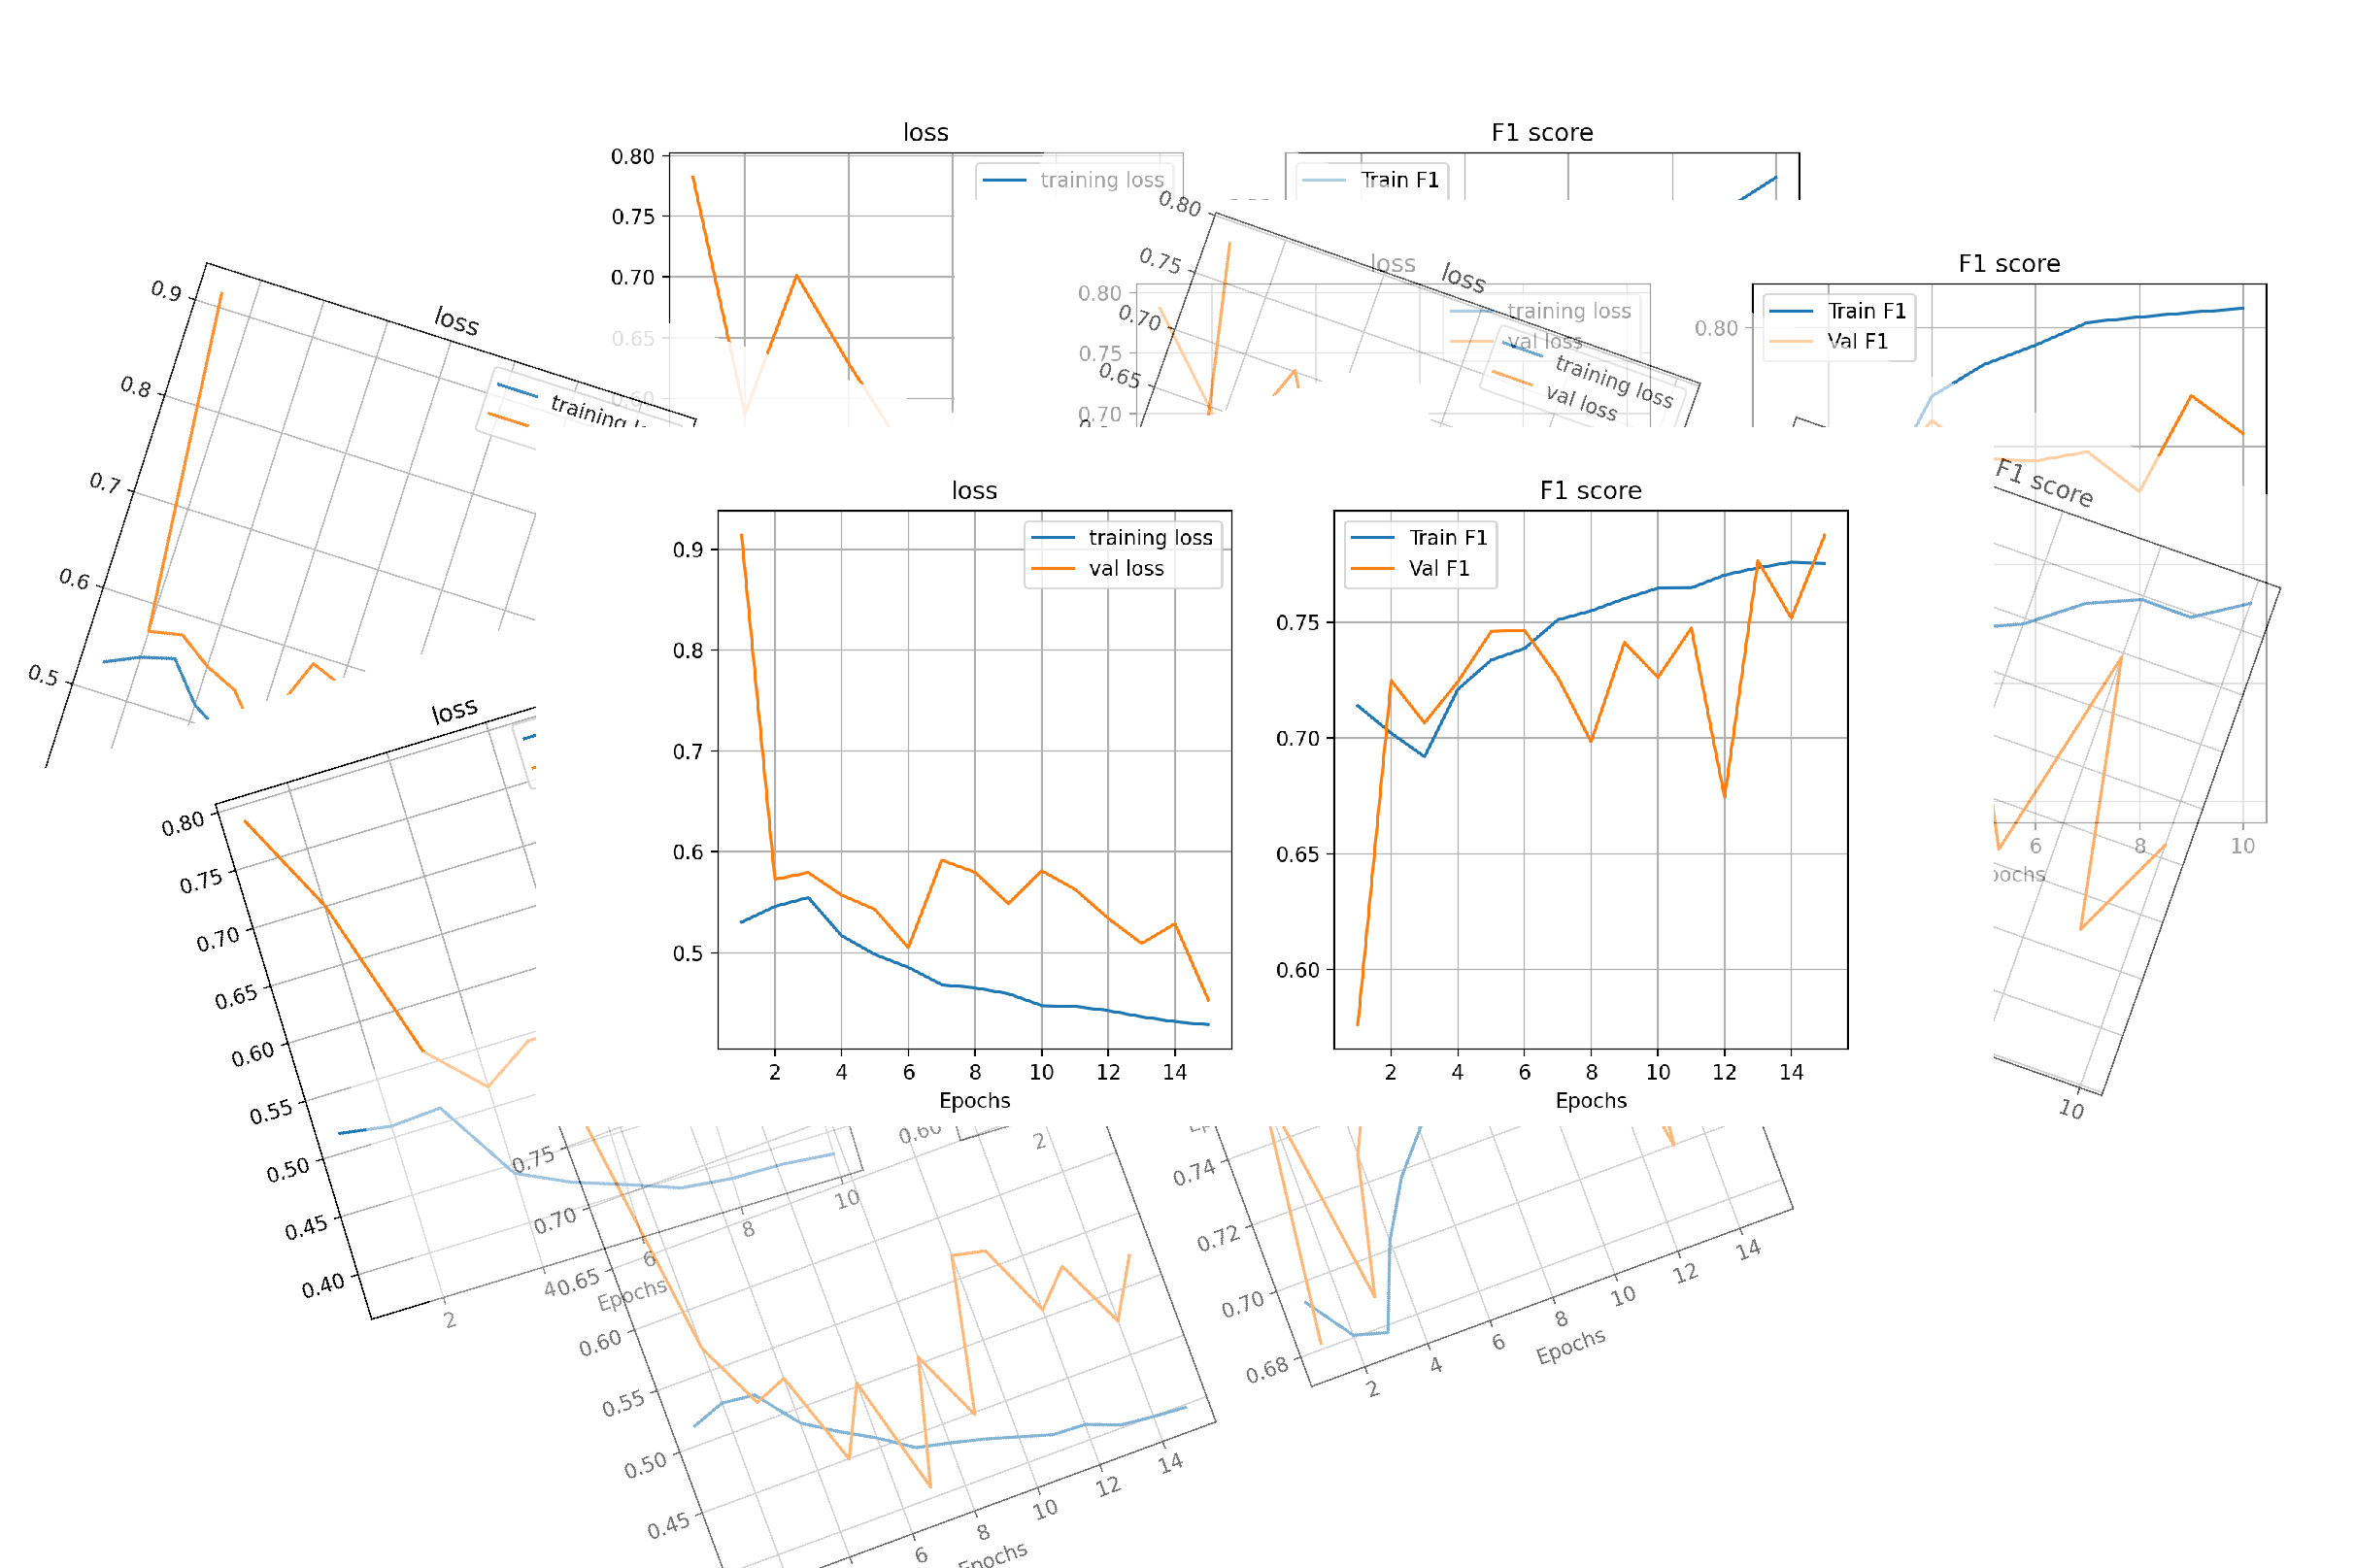
\includegraphics[width=0.8\textwidth]{figures/lotoftraining.pdf}
    \caption{}
    \end{figure}

\end{frame}

%-----EXAMPLE SLIDES-----%

\setbeamertemplate{caption}{\raggedright\insertcaption\par}

\begin{frame}
\frametitle{Results}
\begin{columns}
\begin{column}{0.5\textwidth}

\begin{table}[]
\begin{tabular}{ll}
\hline
\textbf{Model} & \textbf{AUC score} \\ \hline
Transfer Learning & 0.904 \\
Contrastive learning & 0.848 \\ \hline
\end{tabular}
\end{table}

\end{column}
\begin{column}{0.5\textwidth}  %%<--- here
\begin{center}
    \begin{figure}
    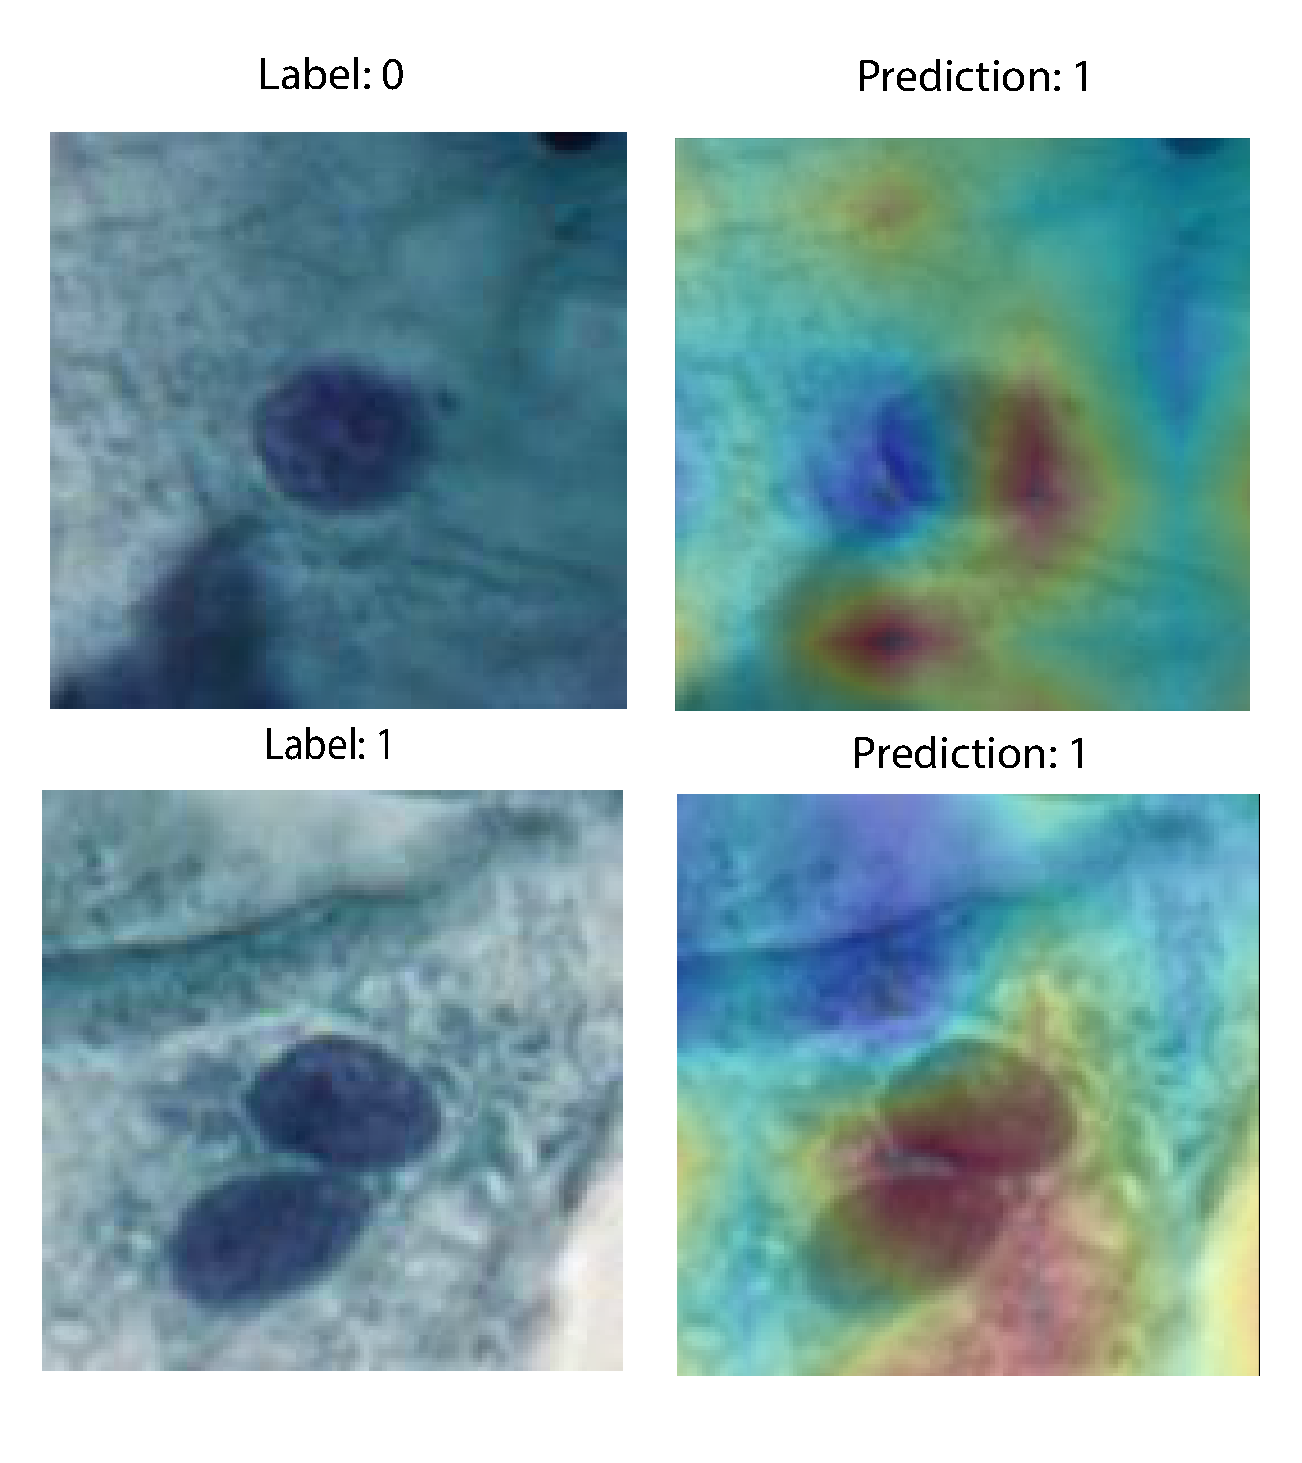
\includegraphics[width=0.8\textwidth]{figures/cam.pdf}
    \caption{CAM generated with the best model}
    \end{figure}
\end{center}
\end{column}
\end{columns}
\end{frame}





% ------------------------------------------------- %


\begin{frame}[allowframebreaks] 
\frametitle{References}
\begin{thebibliography}{1}
\bibitem{SimCL} Ting Chen and
                  Simon Kornblith and
                  Mohammad Norouzi and
                  Geoffrey E. Hinton (2020). A Simple Framework for Contrastive Learning of Visual Representations
\bibitem{} Santisudha Panigrahi and Bhabani Sankar Nanda and Ruchi Bhuyan and Kundan Kumar and Susmita Ghosh and Tripti Swarnkar (2023). Classifying histopathological images of oral squamous cell carcinoma using deep transfer learning

\bibitem{infoloss} Aaron van den Oord and Yazhe Li and Oriol Vinyals (2019). Representation Learning with Contrastive Predictive Coding  
\end{thebibliography}

\end{frame}


\end{document}
